%!TEX root=../talk.tex

\begin{frame}[fragile]
  \frametitle{Proteins}
  \framesubtitle{Biological motivation}

  \begin{columns}
    \begin{column}{0.618\textwidth}
      \vspace{-2em}

      \begin{itemize}
        \item<1-> What are Proteins?
              \begin{itemize}
                \item What do they do?
                \item What are they made of?
              \end{itemize}
        \item<2-> Amino Acids...
              \begin{itemize}
                \item Molecules attract each other,
                \item which results in \textbf{protein folding}.
              \end{itemize}
      \end{itemize}
    \end{column}

    \begin{column}{0.382\textwidth}
      \flushright
      \centering
      \vfill
      \vbox to 0.5\textheight{
        MENFQKVEKIGEGTYGVVYKARNKLT...\\ 
        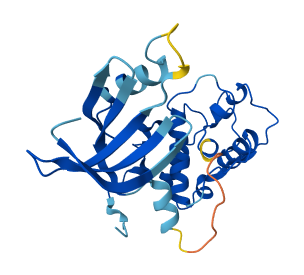
\includegraphics[width=\textwidth]{figs/protein_structure.png}
      }

      {
        \hspace{2em}\\
        \vspace{2em}
        {\footnotesize An example protein and its 3D structure.\footnotemark}
        \par
      }
    \end{column}
  \end{columns}
\footnotetext{Source: AlphaFold DB}
\end{frame}

\begin{frame}[fragile]
  \frametitle{Protein Interactions}
  \framesubtitle{Biological motivation}

  \begin{columns}
    \begin{column}{0.618\textwidth}
      \vspace{-2em}

      \begin{itemize}
        \item<1-> What happens when they collide? \color{WOrchid}Interactions\color{Black}!
              \begin{itemize}
                \item Transient
                \item Obligate
                \item Homo-oligomeric
                \item Hetero-oligomeric
              \end{itemize}
        \item<2-> Interactions enable proteins to act as:
              \begin{itemize}
                \item signals transmitters,
                \item catalysts for chemical reactions,
                \item structural supports for cells, tissues, enzymes, etc.
              \end{itemize}
      \end{itemize}
    \end{column}

    \begin{column}{0.382\textwidth}
      \flushright
      \centering
      \vfill
      \vbox to 0.3\textheight{ 
        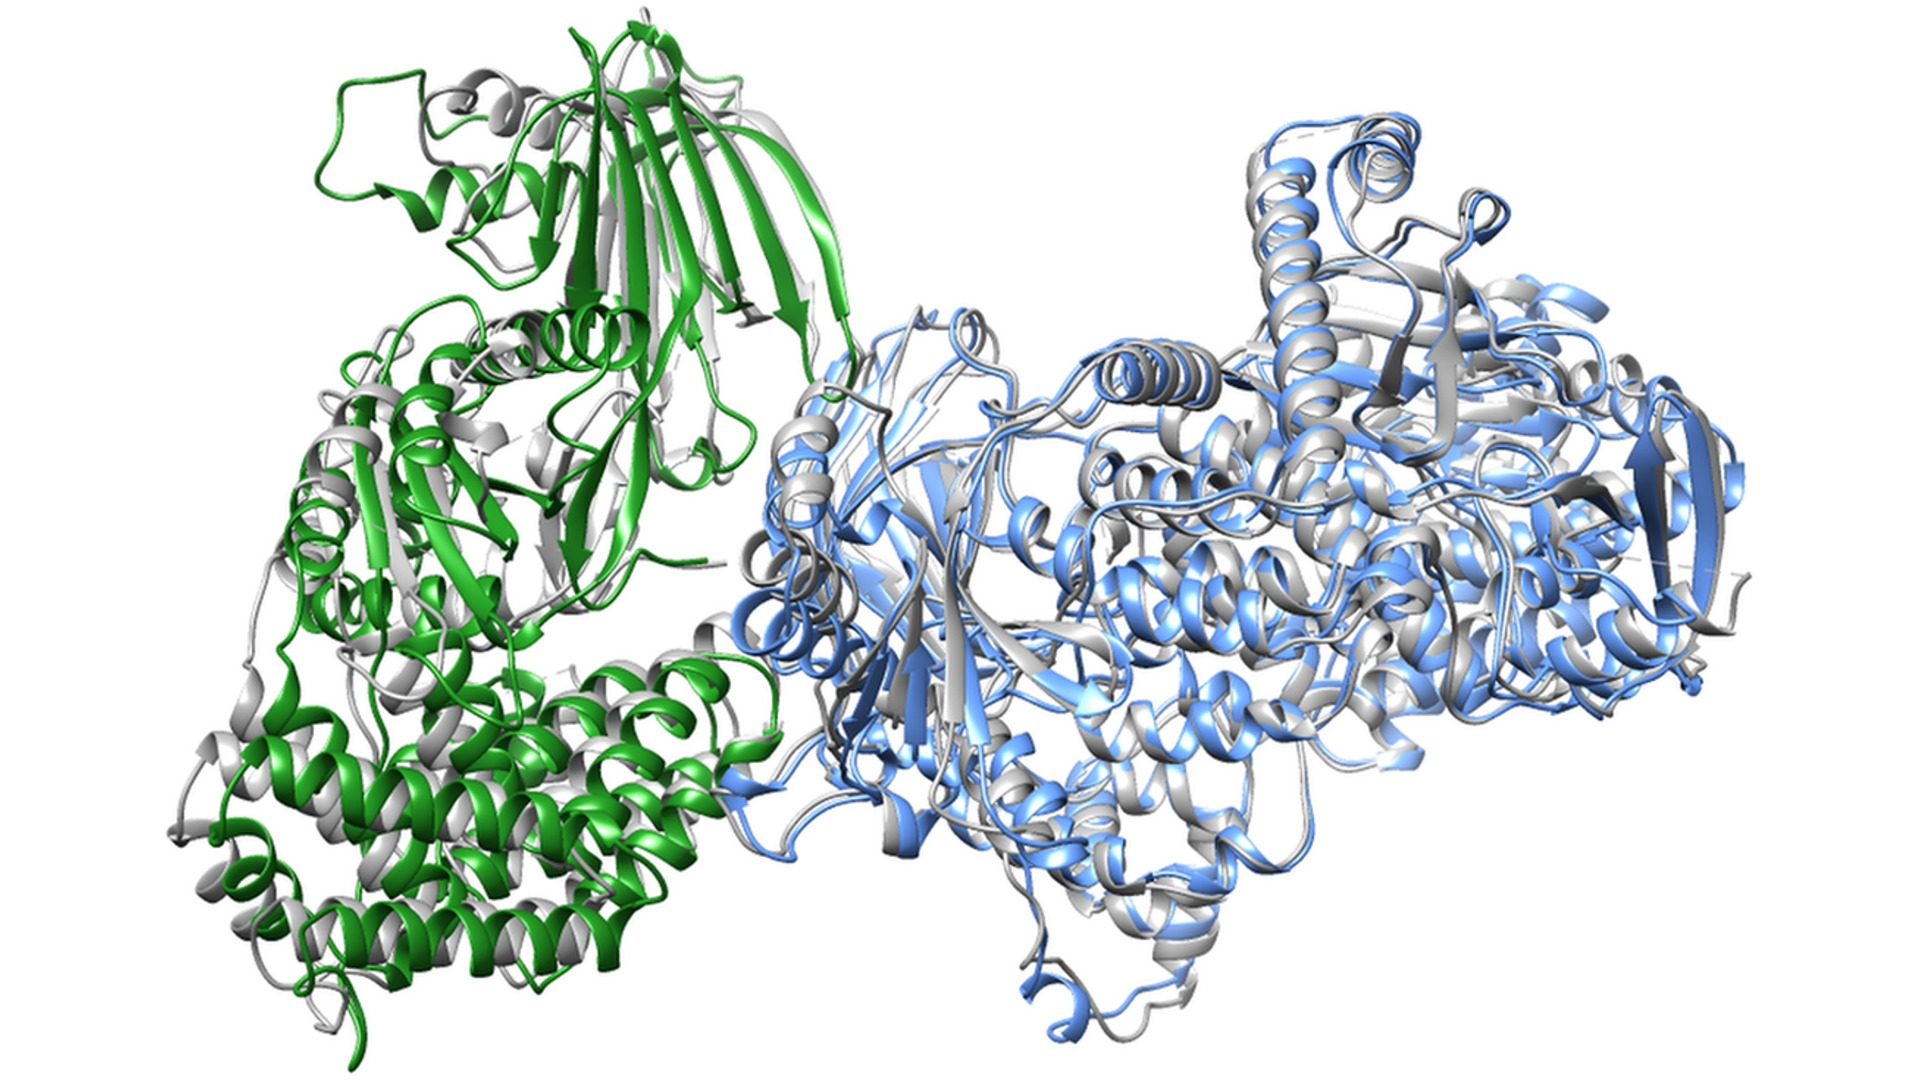
\includegraphics[width=\textwidth]{figs/PPI.jpg}
      }

      {
        \hspace{2em}\\
        {\footnotesize Two proteins interacting \footnotemark }
        \par
      }
    \end{column}
  \end{columns}
\footnotetext{Source: https://www.scilifelab.se/wp-content/uploads/2022/03/Elofsson\_WP.jpg}
\end{frame}

\begin{frame}[fragile]
  \frametitle{Drug Design}
  \framesubtitle{Biological motivation}
      \vspace{-2em}
      \begin{itemize}
        \item<1-> PPIs are drug targets.
              \begin{itemize}
                \item Inhibit cellular regeneration (cancer treatment).
                \item Block disease-causing proteins from interacting with their usual partners.
              \end{itemize}
        \item<2-> How do we know which proteins to target?
        \item<3-> How do we verify that our drug will interact with the target?
      \end{itemize}
\end{frame}

\blackslidetext{
  \centering  
  \Large\bf PPI Detection Methods
}

\begin{frame}[fragile]
  \frametitle{Protein-Protein Interaction Detection}
  \framesubtitle{\textit{in vivo, in vitro}}

  \begin{columns}
    \begin{column}{0.618\textwidth}
      \vspace{-2em}

      \begin{itemize}
        \item<1-> Interactions can be detected using wet lab experiments, e.g.
              \begin{itemize}
                \item Co-immunoprecipitation (Co-IP)
                \item Yeast 2 hybrid (Y2H)
              \end{itemize}
        \item<2-> These methods can be:
              \begin{itemize}
                \item time consuming \tiny [Tang and Takahashi, 2018]\small,
                \item and inaccurate \tiny [Vidalain et al., 2004]\small
              \end{itemize}
      \end{itemize}
    \end{column}

    \begin{column}{0.382\textwidth}
      \flushright
      \centering
      \vfill
      \vbox to 0.5\textheight{ 
        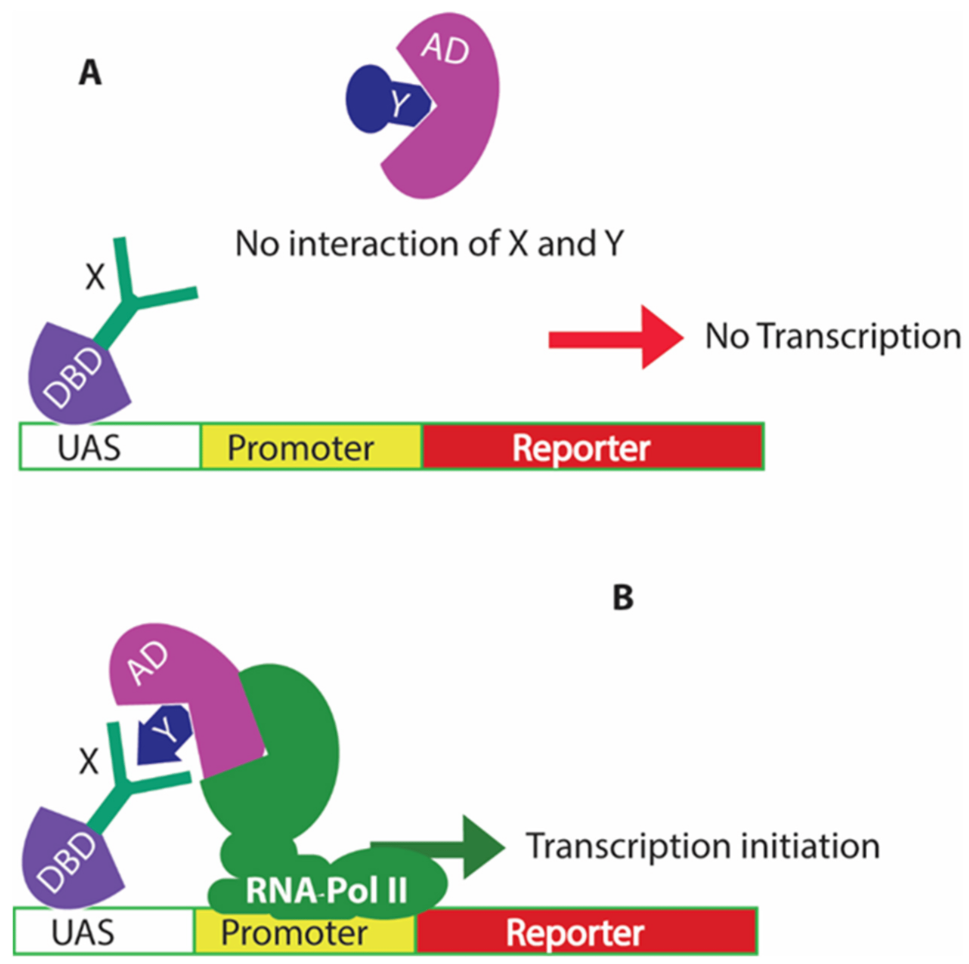
\includegraphics[width=\textwidth]{figs/y2h.png}
      }

      {
        \vspace{2.5em}
        {\footnotesize Y2H screening \footnotemark}
        \par
      }
    \end{column}
  \end{columns}
\footnotetext{Source: https://file.mtoz-biolabs.com/pro/mtoz/20241213/1867402336327553024-yeast-2-hybrid-analysis-service1.png}
\end{frame}

\begin{frame}[fragile]
  \frametitle{Protein-Protein Interaction \underline{Prediction}}
  \framesubtitle{\textit{in silico}}

  \begin{columns}
    \begin{column}{\textwidth}
      \vspace{-2em}

      \begin{itemize}
        \item<1-> What if we predict whether two proteins will interact without the need for wet lab experiments?
              \begin{itemize}
                \item We can use machine learning to model the interaction behaviour of proteins.
              \end{itemize}
        \item<2-> That is the main idea behind the field of PPI prediction.
      \end{itemize}
    \end{column}

    
  \end{columns}

\end{frame}


